\documentclass[twoside]{article}
\usepackage[utf8]{inputenc}
\usepackage[ngerman]{babel}
\usepackage{libertine}
\usepackage[a4paper]{geometry}
\usepackage{parskip}
\usepackage{blindtext}
\usepackage{amsmath, amsthm, amssymb, commath, mathtools}
\usepackage{physics}
\usepackage{nicefrac}
\usepackage{booktabs}
\usepackage{tabularx}
\usepackage{enumitem}
\usepackage{graphicx}
\usepackage{wrapfig}
\usepackage{float}
% \usepackage{minted}
\usepackage{appendix}
\usepackage{icomma}
\usepackage{multirow}
\usepackage{multicol}
\usepackage{footmisc}
\usepackage[separate-uncertainty=true]{siunitx}
\sisetup{locale = DE}

\usepackage{csquotes}
\MakeOuterQuote{"}
\renewcommand{\ttdefault}{cmtt}

\newcommand{\versuch}[0]{STO}

\usepackage{hyperref}
\usepackage{bookmark}
% https://tex.stackexchange.com/a/33701
\makeatletter
    \newcommand{\nonum}[0]{%
        \let\@oldseccntformat\@seccntformat %
        \renewcommand\@seccntformat[1]{}%
        }
    \newcommand{\resnum}[0]{\let\@seccntformat\@oldseccntformat}
\makeatother

\usepackage{chngcntr}
\counterwithin{figure}{section}

\hypersetup{
	pdftitle={P1 -- \versuch{} Auswertung},
	pdfauthor={Yudong Sun},
	bookmarksnumbered=true,
	bookmarksopen=true,
	bookmarksopenlevel=2,
	pdfstartview=Fit,
	pdfpagemode=UseOutlines,
	colorlinks=true,
	linkcolor=black,
	filecolor=magenta,      
	urlcolor=blue
}
\urlstyle{same}

\title{STO -- Stöße \\ Auswertung}
\author{Yudong Sun \\{\small in Zusammenarbeit mit Fabian Solfronk und Simon Pfeiffer}\\\\ Gruppe F2}

\usepackage{fancyhdr}
\pagestyle{fancy}
\fancyhf{}
\fancyhead[RO]{Yudong Sun}
\fancyhead[LO]{Auswertung -- \versuch}
\fancyhead[LE]{Yudong Sun}
\fancyhead[RE]{Auswertung -- \versuch}
\cfoot{\thepage}

% Custom Defs
\newcommand{\ra}[1]{\renewcommand{\arraystretch}{#1}}
\newcommand{\maxi}[1]{\text{max}\left(#1\right)}
\newcommand{\mini}[1]{\text{min}\left(#1\right)}
% / Custom Defs

\begin{document}

\maketitle

% Einstellungen
\nonum
\numberwithin{equation}{section}
% / Einstellungen

\section{Teilversuch 1: Flugweiten und Streuung verschiedener Projektilarten}
    \subsection{Messung}
        Fehler beim Abschlagen des Schienendes auf das Transparentpaper $= \SI{0.5}{\milli\meter}$\\
        Fehler bei Markierung des Aufschlagspunktes $= \SI{1.0}{\milli\meter}$ \\
        Fehler beim Lesen des Lineal $= \SI{0.5}{\milli\meter}$ (beim 0) $+ ~\SI{0.5}{\milli\meter}$ (beim Aufschlagspunkt) $ = \SI{1,0}{\milli\meter}$

        Fehler bei Messung der Flugweiten insgesamt $= \SI{2.5}{\milli\meter}$

        \vspace{\baselineskip}
        \begin{center}
            \ra{1.2}
            \begin{tabular}{l rrrrr r}
                \toprule
                \multirow{2}{*}{Kugelart} & \multicolumn{5}{c}{Flugweite $x_i$ im Versuch $i$ / $\SI{}{\milli\meter}$} & \multirow{2}{*}{~Mittelwert $\bar{x}$} \\
                \cmidrule{2-6} & $1$ & $2$ & $3$ & $4$ & $5$ &  \\
                \midrule
                Kleine Stahlkugel & $\SI{254.0}{}$ & $\SI{252.5}{}$ & $\SI{255.5}{}$ & $\SI{253.0}{}$ & $\SI{255.0}{}$ & $\SI{254.0}{}$\\
                Große Stahlkugel  & $\SI{255.0}{}$ & $\SI{257.5}{}$ & $\SI{253.5}{}$ & $\SI{256.0}{}$ & $\SI{258.0}{}$ & $\SI{256.0}{}$\\
                Glaskugel         & $\SI{239.5}{}$ & $\SI{238.0}{}$ & $\SI{233.0}{}$ & $\SI{245.0}{}$ & $\SI{240.5}{}$ & $\SI{239.2}{}$\\
                Plastikkugel      & $\SI{235.5}{}$ & $\SI{249.5}{}$ & $\SI{264.0}{}$ & $\SI{250.0}{}$ & $\SI{258.0}{}$ & $\SI{251.4}{}$\\
                \bottomrule
            \end{tabular}
        \end{center}
        \vspace{\baselineskip}

        Der Mittelwert $\bar{x}$ wurde wie folgt berechnet:
        \begin{equation}
            \bar{x} = \frac{1}{5} \left(\sum_{x=1}^{5} x_i \right) \label{eqn:mittelwert}
        \end{equation}

        Da alle Messungen stochastisch unabhängig sind, benutzen wir hier die Gauß'scher Fehlerfortpflanzung:
        \begin{equation}
            \Delta \bar{x} = \frac{1}{5} \sqrt{5 \left(\Delta x_i\right)^2} = \frac{1}{5} \sqrt{5 \left(\SI{2.5}{\milli\meter}\right)^2} = \SI{1.1}{\milli\meter}
        \end{equation}

    \subsection{Fehlerkreis}
        Die Fehlerkreise sind auf dem korpierten Transparenzpapier gezeichnet. Circa $\nicefrac{2}{3} \times 5 = 3,\bar{3}$ Punkten müssen in diesem Kreis liegen.

        Die Auftreffspunkten für die kleine Stahlkugel waren leider zu eng zusammen. Das hat zu Schwerigkeiten beim Zeichnen des Fehlerkreises geführt. 

    \subsection{Theoretische Flugweite des kleinen Stahlkugels}
        \newcommand{\sth}[0]{s_{\text{th}}}
        \newcommand{\sexp}[0]{s_{\text{exp}}}

        \subsubsection{Herleitung}
            Aus Gleichung (15) der Anleitung haben wir die Formel für die theoretische Flugweite $\sth$:
            \begin{equation}
                \sth = \sqrt{\frac{4h_1h_2}{1+\frac{2}{5\sin^2 \nicefrac{\beta}{2}}}} = \sqrt{\frac{4h_1\left(h-\varnothing\right)}{1+\frac{2}{5\sin^2 \nicefrac{\beta}{2}}}} = \mu\sqrt{h - \varnothing}
            \end{equation}
            mit
            \begin{center}
                \begin{tabular}{lrl}
                    \toprule
                    Variable & Wert mit Fehler & Bedeutung \\
                    \midrule
                    $h_1$ & \SI{229.0}{\milli\meter} & Höhendifferenz zws. Startposition und Schienenauslauf \\
                    $\beta$ & \SI{120}{\degree} & Öffnungswinkel \\
                    $h$   & \SI{138.00(2)}{\milli\meter} & Höhe von Stahlkugeloberfläsche bis Detektorboden \\
                    $\varnothing$ & \SI{20.00(5)}{\milli\meter} & Durchmesser des Stahlkugels \\
                    \bottomrule
                \end{tabular}
            \end{center}
            \vspace{\baselineskip}

            wobei $h_2 = h' - 2 \times \nicefrac{\varnothing}{2} = h - \varnothing$ die Höhedifferenz zwischen Anfangs- und Endestahlkugelmittelpunkt und $\mu$ der fehlerfreie Vorfaktor von $\sqrt{h - \varnothing}$.

            Der Fehler $\Delta \sth$ ist gegeben durch: 
            \begin{equation}
                \Delta \sth = \sqrt{\left(\pdv{\sth}{h} \Delta h\right)^2 + \left(\pdv{\sth}{\varnothing} \Delta \varnothing\right)^2} \label{eqn:fehler}
            \end{equation}

            Die partielle Ableitungen liefern jeweils:
            \vspace{-\baselineskip}
            \begin{multicols}{2}
                \begin{equation}
                    \pdv{\sth}{h} = \frac{\mu}{2}\left(h-\varnothing\right)^{-\frac{1}{2}} = \frac{\mu}{2\sqrt{h-\varnothing}} \label{eqn:pdvsh}
                \end{equation}
                \begin{equation}
                    \pdv{\sth}{\varnothing} = \frac{\mu}{2}\left(h-\varnothing\right)^{-\frac{1}{2}}(-1) = -\frac{\mu}{2\sqrt{h-\varnothing}} \label{eqn:pdvsd}
                \end{equation}
            \end{multicols}

            \eqref{eqn:pdvsh} und \eqref{eqn:pdvsd} ins \eqref{eqn:fehler} einsetzen:
            \begin{equation}
                \Delta \sth = \left(\frac{\mu}{2\sqrt{h-\varnothing}}\right)\sqrt{\left(\Delta h\right)^2 + \left(\Delta \varnothing \right)^2}
            \end{equation}

        \pagebreak[1]
        \subsubsection{Rechnung}
            Vorfaktor $\mu$:
            \begin{equation}
                \mu = \sqrt{\frac{4h_1}{1+\frac{2}{5\sin^2 \nicefrac{\beta}{2}}}} = \sqrt{\frac{4\left(\SI{229.0}{\milli\meter}\right)}{1+\frac{2}{5\sin^2 \left(\SI{60}{\degree}/\SI{}{\degree}\right)}}}
            \end{equation}

            Wert und Fehler von $\sth$:
            \begin{equation}
                \sth = \mu\sqrt{h - \varnothing} = \sqrt{\frac{4\left(\SI{229.0}{\milli\meter}\right)}{1+\frac{2}{5\sin^2 \left(\SI{60}{\degree}/\SI{}{\degree}\right)}}} \sqrt{\SI{138.00}{\milli\meter} - \SI{20,00}{\milli\meter}} = \SI{265.5036}{\milli\meter}
            \end{equation}

            \begin{align}
                \Delta \sth &= \left(\frac{\mu}{2\sqrt{h-\varnothing}}\right)\sqrt{\left(\Delta h\right)^2 + \left(\Delta \varnothing \right)^2} \notag \\
                &= \sqrt{\frac{4\left(\SI{229.0}{\milli\meter}\right)}{1+\frac{2}{5\sin^2 \left(\SI{60}{\degree}/\SI{}{\degree}\right)}}}\left(2\sqrt{\SI{138.00}{\milli\meter} - \SI{20,00}{\milli\meter}}\right)^{-1} \sqrt{\left(\SI{0,02}{\milli\meter}\right)^2 + \left(\SI{0,05}{\milli\meter} \right)^2} \notag \\
                &= \SI{0.07}{\milli\meter}
            \end{align}

            Daraus folgt: $\sth = \SI{265.50(7)}{\milli\meter}$

    \subsection{Diskussion}
        Gefunden sei: $\sexp = \SI{254.0(11)}{\milli\meter}$ und $\sth = \SI{265.50(7)}{\milli\meter}$

        Fehlerintervall:
        \begin{align*}
            \maxi{\sexp} &= \SI{255.1}{\milli\meter} &&& \maxi{\sth} &= \SI{265.57}{\milli\meter}\\
            \mini{\sexp} &= \SI{252.9}{\milli\meter} &&& \mini{\sth} &= \SI{265.43}{\milli\meter}
        \end{align*}

        $3 \times$ Fehlerintervall:
        \begin{align*}
            \maxi{\sexp} &= \SI{257.3}{\milli\meter} &&& \maxi{\sth} &= \SI{265.71}{\milli\meter}\\
            \mini{\sexp} &= \SI{250.7}{\milli\meter} &&& \mini{\sth} &= \SI{265.29}{\milli\meter}
        \end{align*}

        Das experimentelles Ergebnis $\sexp$ und der theoretische Wert $\sth$ unterscheiden sich signifikant voneinander.

        Dieser Unterschied kann zu 2 Gründe vermütlich zurückgeführt werden:
        \begin{enumerate}
            \item Energieverlust

                Der Energieverlust durch Reibung und andere Faktoren könnte man in dieses Experiment nicht vernachlässigen. Der Stahlkugel könnte deshalb nicht so weit wie erwartet fliegen.

            \item Skalierung aufgrund des Kopierens

                Beim Kopieren kann das Bild trotz der Einstellung skaliert werden. Das führt zu einem systematischen Fehler, den man berücksichtigen muss.
        \end{enumerate}

    \newpage
    \subsection{Reibungskoeffizient $\kappa$}
        Aus der Anleitung ist der Reibungskoeffizient $\kappa$ gegeben durch:
        \begin{equation}
            \kappa = \frac{h_1}{S}\left(1 - \frac{\sexp^2}{\sth^2}\right)
        \end{equation}
        mit 
        \begin{center}
            \begin{tabular}{lrl}
                \toprule
                Variable & Wert mit Fehler & Bedeutung \\
                \midrule
                $h_1$ & \SI{229.0}{\milli\meter} & Höhendifferenz zws. Startposition und Schienenauslauf \\
                $S$   & \SI{728}{\milli\meter}   & Bahnlänge der Schiene \\
                $\sexp$ & \SI{254.0(11)}{\milli\meter} & Flugweite (Experimentell) \\
                $\sth $ & \SI{265.50(7)}{\milli\meter} & Flugweite (Theoretisch) \\
                \bottomrule
            \end{tabular}
        \end{center}
        \vspace{\baselineskip}

        \subsubsection{Herleitung des Fehlers}
            Der Fehler $\Delta \kappa$ ist gegeben durch: 
            \begin{equation}
                \Delta \kappa = \sqrt{\left(\pdv{\kappa}{\sexp} \Delta \sexp\right)^2 + \left(\pdv{\kappa}{\sth} \Delta \sth\right)^2} \label{eqn:kfehler}
            \end{equation}

            Die partielle Ableitungen liefern jeweils:
            \vspace{-\baselineskip}
            \begin{multicols}{2}
                \begin{equation}
                    \pdv{\kappa}{\sexp} = \frac{h_1}{S}\left(-\frac{2\sexp}{\sth^2}\right) = \frac{2h_1}{S}\left(-\frac{\sexp}{\sth^2}\right) \label{eqn:pdvke}
                \end{equation}

                \begin{equation}
                    \pdv{\kappa}{\sth} = \frac{h_1}{S}\left(2\sexp^2\sth^{-3}\right) = \frac{2h_1}{S}\left(\frac{\sexp^2}{\sth^3}\right) \label{eqn:pdvkt}
                \end{equation}
            \end{multicols}

            \eqref{eqn:pdvke} und \eqref{eqn:pdvkt} ins \eqref{eqn:kfehler} einsetzen:
            \begin{equation}
                \Delta \kappa = \left(\frac{h_1}{S}\right)\left(\frac{2\sexp}{\sth^2}\right)\sqrt{\left(\Delta \sexp\right)^2 + \left(\frac{\sexp}{\sth}\Delta \sth \right)^2}
            \end{equation}
        \subsubsection{Rechnung}
            \begin{align}
                \kappa &= \frac{h_1}{S}\left(1 - \frac{\sexp^2}{\sth^2}\right) = \frac{\SI{229.0}{\milli\meter}}{\SI{728}{\milli\meter}}\left(1 - \frac{\left(\SI{254.0}{\milli\meter}\right)^2}{\left(\SI{265.50}{\milli\meter}\right)^2}\right)\notag \\
                & = \SI{2.66599e-2}{} \\
                \Delta \kappa &= \left(\frac{h_1}{S}\right)\left(\frac{2\sexp}{\sth^2}\right)\sqrt{\left(\Delta \sexp\right)^2 + \left(\frac{\sexp}{\sth}\Delta \sth \right)^2} \notag \\
                &= \frac{\SI{229.0}{\milli\meter}}{\SI{728}{\milli\meter}}\left(\frac{2\times\SI{254.0}{\milli\meter}}{\left(\SI{265.50}{\milli\meter}\right)^2}\right) \sqrt{\left(\SI{1.1}{\milli\meter}\right)^2 + \left(\frac{\SI{254.0}{\milli\meter}}{\SI{265.50}{\milli\meter}}\SI{0.07}{\milli\meter} \right)^2} \notag \\
                &= \SI{2.5e-3}{}
            \end{align}

            Daraus folgt: $\kappa = \SI{2.67(25)e-2}{}$. $\kappa$ ist einheitslos.

\section{Teilversuch 2: Elastischer Stoß von Kugeln gleicher Masse}
    \begin{wrapfigure}{i}{0.4\textwidth}
        \begin{center}
            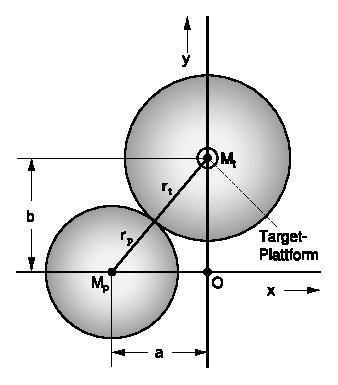
\includegraphics[width=0.25\textwidth]{kugelkorrektur.eps}
        \end{center}
        \caption{Abbildung aus Skript für die Korrektur die Auftreffspunkte auf dem Detektorboden. \vspace{-3\baselineskip}}
    \end{wrapfigure}

    Der Punkt $O$ ist der Schnittpunkt zwischen der $b = 0$ Linie und der dazu senkrechten Linie, die durch die Target-Plattform gerichtet ist. Das heißt, Punkt $O$ ist $20 + 5 = \SI{25}{\milli\meter}$ vom Schienenende entfernt. Er ist mit schwarzem Stift auf dem kopierten Experimentierpapier gezeichnet. 

    Da die Kugeln endlichen Radien haben, müssen die Landepunkte dementsprechend korrigiert werden sein, sodass die gemisste Flugbahnen wirklich die theoretische Flugbahn entspricht. 

    Man kann zur Korrektur wie folgt machen:
    \begin{itemize}
        \item Landepunkt des Targets um die Strecke $b$ in der negativer $y$-Richtung schieben.
        \item Landepunkt des Projektil um die Strecke $a$ in der positiver $x$-Richtung schieben.
    \end{itemize}
    wobei die Strecke $a$ durch diese Formel gegeben ist: $a = \sqrt{\left(r_p + r_t\right)^2 - b^2}$

    Diese Korrektur reicht aber in diesen Fall nicht aus. Nachdem die Projektilkugel der Schienenende verlassen hast, fängt sie sofort an, zu fallen. Das passiert bevor die Projektilkugel die Targetkugel trifft. Dieser schiefer Auftreffwinkel ergibt die Targetkugel nicht nur eine horizontale Anfangsgeschwindigkeit, sondern auch eine nicht vernachlässigbare Anfangsgeschwindigkeit nach oben. Die Flugweite beider Kugeln ändern sich dadurch. 

    Man braucht großen Aufwand, um diese Änderung zu korrigieren, und deshalb wurde es in diesem Versuch nicht berücksichtigt. 

    \subsection{Messung der Flugweite}
        Fehler beim Abschlagen des Schienendes auf das Transparentpaper $= \SI{0.5}{\milli\meter}$\\
        Fehler bei Markierung des Punktes $O$ $ = \SI{1,0}{\milli\meter}$ \\
        Fehler bei Markierung des Aufschlagspunktes $= \SI{1.0}{\milli\meter}$\\
        Fehler beim Lesen des Lineal $= \SI{0.5}{\milli\meter}$ (beim 0) $+ ~\SI{0.5}{\milli\meter}$ (beim Aufschlagspunkt) $ = \SI{1,0}{\milli\meter}$

        \textbf{Fall} $b = 0$ \textbf{:}

        Fehler bei Messung der Flugweiten für $b = 0$ insgesamt $= \SI{4.5}{\milli\meter}$

        \begin{center}
            \ra{1.2}
            \begin{tabular}{rrrrr r}
                \toprule
                \multicolumn{5}{c}{Flugweite $x_i$ im Versuch $i$ / $\SI{}{\milli\meter}$} & \multirow{2}{*}{~Mittelwert $\bar{x}$} \\
                \cmidrule{1-5} $1$ & $2$ & $3$ & $4$ & $5$ &  \\
                \midrule
                $\SI{228.0}{}$ & $\SI{228.5}{}$ & $\SI{230.0}{}$ & $\SI{231.5}{}$ & $\SI{233.0}{}$ & $\SI{230.2}{}$\\
                \bottomrule
            \end{tabular}
        \end{center}
        Der Mittelwert $\bar{x}$ wurde wie in \eqref{eqn:mittelwert} berechnet.

        Ein Kreis mit einem Durchmesser von $\varnothing = \SI{230.2}{\milli\meter} \equiv \SI{230}{\milli\meter}$ war auf dem korpiertem Experimentierpapier für den nächsten Teil der Auswertung zum Teilversuch 2 gezeichnet.

        \pagebreak
        \textbf{Fall} $b \neq 0$ \textbf{:}

        Fehler bei Markierung des Abstands $b$ bzw. $a$ von Punkt $O$ $= \SI{1.0}{\milli\meter}$ 

        Fehler bei Messung der Flugweiten für $b \neq 0$ insgesamt $= \SI{4.5}{\milli\meter}$

        Für die Targetkugel:
        \begin{center}
            \begin{tabular}{l rrrrrrrrrr}
                \toprule
                \multirow{2}{*}{$n$~} & \multicolumn{10}{c}{Flugweite $x_{in}$ mit Stoßparameter $\left(b_i/\SI{}{\milli\meter}\right)$ / $\SI{}{\milli\meter}$}  \\
                \cmidrule{2-11} & $3$ & $4$ & $6$ & $9$ & $12$ & $15$ & $17$ & $18$ & $19$ & $19,5$ \\
                \midrule
                $1$ & $260,0$ & $258,0$ & $250,0$ & $238,0$ & $206,0$ & $169,0$ & $131,0$ & $105,0$ & $64,0$ & $43,0$ \\
                $2$ & $261,0$ & $260,0$ & $253,0$ & $238,0$ & $208,0$ & $172,0$ & $133,0$ & $108,0$ & $72,0$ & $46,0$ \\
                $3$ & $263,0$ & $259,0$ & $254,0$ & $238,0$ & $207,0$ & $173,0$ & $134,0$ & $109,0$ & $73,0$ & $48,0$ \\
                \midrule
                $\bar{x_i}$ & $261,3$ & $259,0$ & $252,3$ & $238,0$ & $207,0$ & $171,3$ & $132,7$ & $107,3$ & $69,7$ & $45,7$ \\
                \bottomrule
            \end{tabular}
        \end{center}
        \vspace{0.5\baselineskip}

        Für die Projektilkugel:
        \begin{center}
            \begin{tabular}{l r rrrrrrrrrr}
                \toprule
                && \multicolumn{10}{c}{Flugweite $x_{in}$ mit Parameters / $\SI{}{\milli\meter}$}  \\
                \cmidrule{3-12} & $\left(b_i/\SI{}{\milli\meter}\right)$ & $3$ & $4$ & $6$ & $9$ & $12$ & $15$ & $17$ & $18$ & $19$ & $19,5$ \\
                $n$ & $\left(a_i/\SI{}{\milli\meter}\right)$ & $19,8$ & $19,6$ & $19,1$ & $17,9$ & $16,0$ & $13,2$ & $10,5$ & $8,7$ & $6,2$ & $4,4$ \\
                \midrule
                $1$ &  & - & - & $79,0$ & $111,0$ & $154,0$ & $184,0$ & $205,0$ & $214,0$ & $222,0$ & $228,0$ \\
                $2$ &  & - & - & $81,0$ & $113,0$ & $153,0$ & $181,0$ & $205,0$ & $212,0$ & $222,0$ & $228,0$ \\
                $3$ &  & - & - & $80,0$ & $116,0$ & $152,0$ & $181,0$ & $202,0$ & $212,0$ & $224,0$ & $229,0$ \\
                \midrule
                & $\bar{x_i}$ & - & - & $80,0$ & $113,3$ & $153,0$ & $182,0$ & $204,0$ & $212,7$ & $222,7$ & $228,3$ \\
                \bottomrule
            \end{tabular}
        \end{center}
        \vspace{0.5\baselineskip}
        wobei $n$ die Versuchsnummer ist. Die Mittelwerte $\bar{x_i}$ wurden analog zu \eqref{eqn:mittelwert} berechnet (mit $3$ statt $5$).

        \subsection{Fehlermessung}
            \subsubsection{Direkte Messung}
            Ohne Korrektur für die Strecke $a$ und $b$ wurden die Fehler gemessen. Diese Messung entspricht den kürzesten Abstand zwischen einem Punkt und dem Kreisumfang. Wir bezeichnen einen Fehler eines Punktes als positv, wenn dieser Punkt außerhalb des Kreises liegt. Der Fehler bei dieser Fehlermessung ist der gleiche wie bei dem Fall $b \neq 0$. 

            Es gibt keinen Zusammenhang zwischen der Versuchsnummer dieser Fehlermessung und der der vorherigen Flugweitemessung.

            Für die Targetkugel:
            \begin{center}
                \begin{tabular}{l rrrrrrrrrr}
                    \toprule
                    \multirow{2}{*}{$n$~} & \multicolumn{10}{c}{Fehler $y_{in}$ mit Stoßparameter $\left(b_i/\SI{}{\milli\meter}\right)$ / $\SI{}{\milli\meter}$}  \\
                    \cmidrule{2-11} & $3$ & $4$ & $6$ & $9$ & $12$ & $15$ & $17$ & $18$ & $19$ & $19,5$ \\
                    \midrule
                    $1$ & $33,5$ & $33,0$ & $32,0$ & $33,0$ & $24,0$ & $22,0$ & $15,0$ & $10,0$ & $7,0$ & $3,5$ \\
                    $2$ & $34,0$ & $34,0$ & $34,0$ & $33,0$ & $26,0$ & $22,0$ & $15,0$ & $11,5$ & $7,0$ & $4,0$ \\
                    $3$ & $36,0$ & $35,0$ & $35,0$ & $33,0$ & $24,0$ & $20,0$ & $14,0$ & $11,0$ & $5,0$ & $6,0$ \\
                    \midrule
                    $\bar{y_i}$ & $34,5$ & $34,0$ & $33,7$ & $33,0$ & $24,7$ & $21,3$ & $14,7$ & $10,8$ & $6,3$ & $4,5$ \\
                    \bottomrule
                \end{tabular}
            \end{center}
            \vspace{0.5\baselineskip}

            Für die Projektilkugel:
            \begin{center}
                \begin{tabular}{l rrrrrrrrrr}
                    \toprule
                    \multirow{2}{*}{$n$~} & \multicolumn{10}{c}{Fehler $y_{in}$ mit Stoßparameter $\left(b_i/\SI{}{\milli\meter}\right)$ / $\SI{}{\milli\meter}$}  \\
                    \cmidrule{2-11} & $3$ & $4$ & $6$ & $9$ & $12$ & $15$ & $17$ & $18$ & $19$ & $19,5$ \\
                    \midrule
                    $1$ & - & - & $16,0$ & $12,0$ & $12,0$ & $4,0$ & $0,0$ & $0,0$ & $-3,0$ & $-2,0$ \\
                    $2$ & - & - & $17,0$ & $13,0$ & $12,5$ & $4,0$ & $1,0$ & $-3,0$ & $-3,0$ & $-3,0$ \\
                    $3$ & - & - & $17,0$ & $15,0$ & $12,0$ & $5,0$ & $2,0$ & $-3,0$ & $-2,0$ & $-2,5$ \\
                    \midrule
                    $\bar{y_i}$ & - & - & $16,7$ & $13,3$ & $12,2$ & $4,3$ & $1,0$ & $-2,0$ & $-2,7$ & $-2,5$ \\
                    \bottomrule
                \end{tabular}
            \end{center}
            % \vspace{0.5\baselineskip}

        \subsubsection{Mithilfe Daten der Messung der Flugweite}
            Wir können auch die Fehler messen, indem wir die geometrische Eigenschaften eines Kreises zu Nutze machen. Da die Winkel zwischen der Trajektorie zweier gleichen Kugeln immer \SI{90}{\degree} entspricht, soll der Satz des Pythagoras gelten. Sei $s_t$ die Flugweite der Target-Kugel in Millimeter und $s_p$ die Flugweite der Projektil-Kugel in Millimeter, dann gilt es:
            \begin{equation}
                \sqrt{s_t^2 + s_p^2} = \text{Durchmesser des Kreises} = \SI{230.2}{\milli\meter}
            \end{equation}
            Der Fehler ist dann:
            \begin{equation}
                \Delta s = \sqrt{s_t^2 + s_p^2} - \SI{230.2}{\milli\meter}
            \end{equation}
            Tabuliert:
            \begin{center}
                \begin{tabular}{l rrrrrrrrrr}
                    \toprule
                    $b / \SI{}{\milli\meter}$ & $3$ & $4$ & $6$ & $9$ & $12$ & $15$ & $17$ & $18$ & $19$ & $19,5$ \\
                    \midrule
                    $\Delta s / \SI{}{\milli\meter}$ & - & - & $34,7$ & $33,6$ & $27,4$ & $20,0$ & $13,3$ & $8,2$ & $3,3$ & $2,9$ \\
                    \bottomrule
                \end{tabular}
            \end{center}

    \subsection{Diskussion}
        Es ist offentsichlich aus der direkte Messung der Fehler für die Targetkugel und der Pythagoreische Methode, dass der Fehler deutlich abnimmt mit wachsendem Stoßparameter $b$. Bei der Projektilkugel ist der absolute Fehler bei der direkte Messung das kleinste, wenn $b = 17$.

        Wenn die Massen von Projektil und Target unterschiedlich sind, werden die Kugeln auf Kreisen mit verschiedenem Radien landen. Die Kreisradien haben die folgenden Relation:
        \begin{equation}
            \frac{R_p}{R_t} = \frac{m_t}{m_p}
        \end{equation}
        Sei $P$ die Projektilkugel und $T$ die Targetkugel. Die Stöße werden dann zum Beispiel so aussehen:
        \begin{figure}[H]
            \centering
            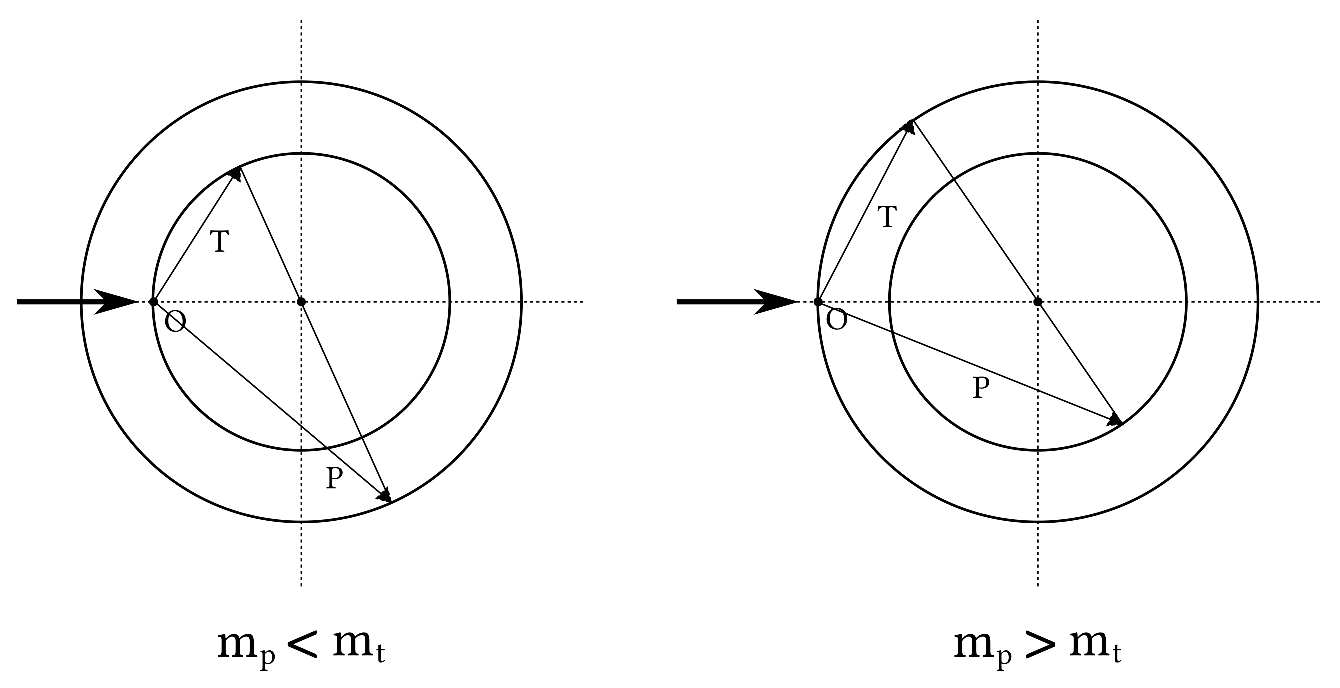
\includegraphics[width=0.5\textwidth]{diffmass.eps}
            \caption{Ortskurven für elastische Stöße bei verschiedenen Massenrelationen}
        \end{figure}
        Die Flugbahnen werden natürlich vom Stoßparameter $b$ abhängen. Die Winkel $\gamma$ zwischen der beiden Pfaden wird auch von \SI{90}{\degree} abweichen: $m_p < m_t \implies \gamma > \SI{90}{\degree}$ und $m_p > m_t \implies \gamma < \SI{90}{\degree}$.

        Die Fehler der Werten wurden in dieser Diskussion nicht berücksichtigt.  

\section{Teilversuch 3: Bewegungsanalyse mit Hochgeschwindigkeitskamera}
    Siehe Protokoll für das erste Teil der Auswertung zum Teilversuch 3.

    \subsection{Theoretische Werte}
        \subsubsection{Beschleunigung $a$}
            Aus Gleichung (4) der Anleitung ist $a$ gegeben durch:
            \begin{equation}
                a = \frac{g \sin \alpha}{1 + \displaystyle \frac{\rule{0pt}{1em} 2}{5 \sin^2 \nicefrac{\beta}{2}}}
            \end{equation}
            mit
            \begin{center}
                \begin{tabular}{lrl}
                    \toprule
                    Variable & Wert & Bedeutung \\
                    \midrule
                    $g$ & \SI{9.807}{\meter\per\second\squared} & Erdfeldbeschleunigung \\
                    $\alpha$ & \SI{37}{\degree} & Neigungswinkel der schiefen Ebene \\
                    $\beta$ & \SI{120}{\degree} & Öffnungswinkel \\
                    \bottomrule
                \end{tabular}
            \end{center}
            Das heißt: 
            \begin{equation}
                a = \frac{\SI{9.807}{\meter\per\second\squared} \times \sin \left(\SI{37}{\degree} / \SI{}{\degree}\right)}{1 + \displaystyle \frac{\rule{0pt}{1em} 2}{5 \sin^2 \left(\SI{60}{\degree}/\SI{}{\degree}\right)}} = \SI{3.8}{\meter\per\second\squared} \text{~~~~(2 sig. Zif.)}
            \end{equation}

        \subsubsection{Abfluggeschwindigkeit $u$}
            Aus Gleichung (10) der Anleitung ist $u$ gegeben durch:
            \begin{equation}
                u = \sqrt{\frac{2gh_1}{1 + \displaystyle \frac{\rule{0pt}{1em} 2}{5 \sin^2 \nicefrac{\beta}{2}}}}
            \end{equation}
            mit
            \begin{center}
                \begin{tabular}{lrl}
                    \toprule
                    Variable & Wert & Bedeutung \\
                    \midrule
                    $h_1$ & \SI{229.0}{\milli\meter} & Höhendifferenz zws. Startposition und Schienenauslauf \\
                    $g$ & \SI{9.807}{\meter\per\second\squared} & Erdfeldbeschleunigung \\
                    $\beta$ & \SI{120}{\degree} & Öffnungswinkel \\
                    \bottomrule
                \end{tabular}
            \end{center}
            Das heißt:
            \begin{equation}
                u = \sqrt{\frac{2\times \SI{9.807}{\meter\per\second\squared} \times \SI{229.0e-3}{\meter}}{1 + \displaystyle \frac{\rule{0pt}{1em} 2}{5 \sin^2 \left(\SI{60}{\degree}/\SI{}{\degree}\right)}}} = \SI{1.7}{\meter\per\second} \text{~~~~(2 sig. Zif.)}
            \end{equation}

    \subsection{Vergleich und Diskussion}
        \begin{center}
            \begin{tabular}{lllll}
                \toprule
                Variable & Theorie & Experiment & Abs. Fehler & \% Fehler \\
                \midrule
                $a$ & $\SI{3.8}{\meter\per\second\squared}$ & $\SI{3,544}{\meter\per\second\squared}$ & $\SI{0.3}{\meter\per\second\squared}$ & \SI{6.7}{\percent}\\
                $u$ & $\SI{1.7}{\meter\per\second}$ & $\SI{1.642}{\meter\per\second}$ & $\SI{0.1}{\meter\per\second}$ & \SI{3.4}{\percent} \\
                $g$ & $\SI{9.807}{\meter\per\second\squared}$ & $\SI{9.408}{\meter\per\second\squared}$ & $\SI{0.399}{\meter\per\second\squared}$ & \SI{4.069}{\percent} \\
                \bottomrule
            \end{tabular}
        \end{center}
        wobei der absolute bzw. prozentuale Fehler einer Variable $v$ sich wie folgt berechnen lässt:
        \begin{align}
            \text{Abs. Fehler} = \lvert v_{\text{th}} - v_{\text{exp}} \rvert && \text{\% Fehler} = \frac{\lvert v_{\text{th}} - v_{\text{exp}}\rvert}{v_\text{th}} 
        \end{align}

        Es ist offentsichlich, dass alle experimentelle Werte geringer als ihre theoretische Werte sind. Der Fehler bei $a$ ist auch großer als die bei $u$ und $g$. Das heißt vor allem, dass hier die Situation des nicht rutschfreien Rollens nicht betrifft. 

        Diese Abweichung kann man in zwei Arten umfassen:
        \begin{enumerate}
            \item Abweichungen wegen physikalischer Gründe

                Energieverlust durch Reibung ist in diesem Fall relativ signifikant. Die benutzte Stahlkugel könnte auch wegen mehrfacher Stoßen beschädigt werden. Diesen Faktoren führen zu einem geringeren Wert von $a$, $u$ und $g$.

            \item Abweichungen wegen menschlischer Gründe

                Bei Analyse der Hochgeschwindigkeitsaufnahmen, muss man Punkten und Achsen manuell definieren. Das ist eher ungenau und kann zu Abweichungen führen. 
        \end{enumerate}
% \resnum
% \appendix
\end{document}
